\documentclass[twocolumn,showpacs,
  nofootinbib,aps,superscriptaddress,
  eqsecnum,prd,notitlepage,showkeys,10pt]{revtex4-1}
\usepackage{amsmath}
\usepackage{graphicx}
\usepackage{dcolumn}
\usepackage{hyperref}
\usepackage{float}
% \usepackage{subfigure}
\usepackage{subcaption}
\usepackage{caption}
\usepackage{todo}
\begin{document}

\title{Traversability Estimation with Dynamic Graph CNN}
\author{Francesco Saverio Zuppichini}
\affiliation{Universita della Svizzera Italiana (USI) \\ \texttt{zuppif@usi.ch}}
\begin{abstract}
  Recent deep learning breakthrough allows to effective classify and segment point clouds by converting them into graphs and feed them to \emph{Geometric Deep Learning} models. Point clouds are able to represent any shape in space making them one of the most versatile data-structure for non-euclidean data. The architecture that archives \emph{state of the art} results in booth classify and segment those cloud is Dynamic Graph CNN \cite{dgcnn}. It utilizes a special Convolution operator applied directly on the graph's edge called \emph{EdgeConv} using booth local and global information. The aim of this project is to first reproduce the results on the famous ModelNet40 \cite{shapenet} dataset with more than ten thousand meshed. Reproducing the paper's results ensure our architecture's correctness.
  Then, we test DGCNN against a vanilla CNN on a dataset composed by heightmaps, images where each pixel is the height value of a terrain region, labeled as traversable or not traversable. Those images were generated letting a legged crocodile-like robot, \emph{Krock}, walking into a simulated environment on synthetic maps and cropping the corresponding terrain patch around each stored trajectory pose. This dataset represents a really interesting playground to explore which architecture is able to extract the most information from the geometry of the terrain and correctly predict their traversability. 
\end{abstract}
\maketitle
\section{Introduction}

Graphs can express a wide array of data structures using a set of nodes and the relationship between them, edges. Graphs are non-euclidean data, thus standard deep learning methods, like CNN \cite{cnn}, fails. Recently, a new set of machine learning models, \emph{Graph Deep Learning} have flourished and successfully applied on a wide array of graphs structure such as social networks, proteins, and on point clouds. A Point cloud is a set of data points in space that often represents a specific 3D object by defined its points coordinates. They are extremely flexible and can be easily gather using consumer hardware such as a Kinect or a Lidar. Even if they are not graphs by definition, we can easily convert them connecting to each point $k$ neighbors.

As with images, we are interested in classify of segment those point clouds. The current architecture that achieves the \emph{state of the art} in those tasks is \emph{Dynamic Graph CNN} proposed by Wang et all \cite{dgcnn}. It utilizes a special convolution layer,  \emph{EdgeConv}, to classify or segment point clouds. 

This project will focus on explaining, test and evaluate this architecture. First, we will reproduce the results of the original paper on the classification task. Then to test its effectiveness on predicting traversability estimation using ground's patches for a legged robot by comparing it to a classic CNN approach. The discussion will only scrape the surface of the topic and will not treat in detail other architectures. If interested, we suggest to the reader the review by Zhou et all \cite{1812.08434}.
\subsection{Method}
In this section we summarized the original paper's proposed architectures using a bottom-up approach.
\subsection{Dynamic Graph CNN}
Dynamic Graph CNN is composed of multiple layers of \emph{EdgeConv} stacked one after the other similar to how convolutions are integrated into CNN. Figure \ref{fig : DGCNN} shows the two architecture proposed by the Authors, for classification and segmentation. 
\begin{figure*}
  \centering
  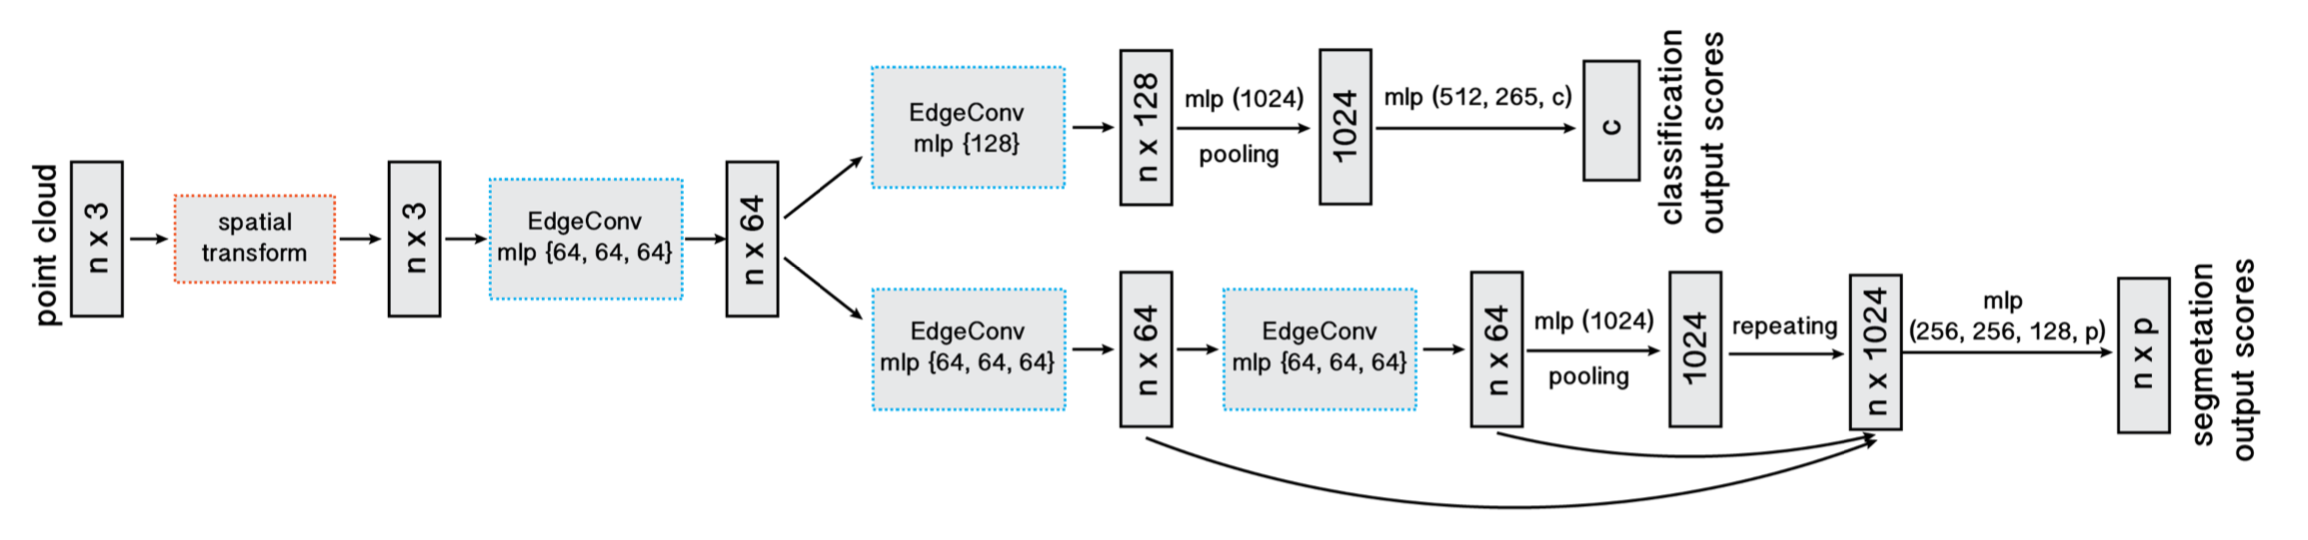
\includegraphics[width=\linewidth]{images/DGCNN.png}
\caption{The two Dynamic Graph CNN architectures divided into an upper and lower branch for classification and segmentation respectively, image from the original paper \cite{dgcnn}. In each edge conv, mlp$\{n_0, ..., n_{i}\}$ represents the number of output neurons of each dense layer. For example, in the first edge conv there are three dense layers with outputs size of $64$.}
\label{fig : DGCNN}
\end{figure*}
\subsubsection{EdgeConv}
Given a point cloud with $n$ denoded as $X=\left\{x_{1}, \ldots, x_{n}\right\} \subseteq R^{F}$ and a graph $\mathcal{G}=(\mathcal{V}, \mathcal{E})$ representing the local structure of the cloud, the $i$-th output of \emph{EdgeConv} operation is defined as
\begin{equation}
  x_{i}^{\prime}=\square_{j :(i, j) \in \mathcal{E}} h_{\Theta}\left(x_{i}, x_{j}\right)
  \end{equation}
Where $\square$ is a channel wise aggregation function and $h_{\Theta}$ is the edge function. The authors choose $\square=max$ and $h_{\Theta} = h_{\Theta}(x_i, x_j - x_i)$. Where $x_i$ and $x_j$ are the coordinates of the center of the patch and its neighbors respectively. Intuitivelly, this allows the layer to use booth global and local information about the mesh. In addition, the edge function has a learnable parameter $\Theta$ that is a classic feed-forward neural network. 
\subsubsection{Dynamic EdgeConv}
The authors shows that dynamically recompute the graph using k-nearest neighbors algorithm improves performance. Thus, the \emph{DynamicEdgeConv} $i$-th output at layer $l$ is defined as:

\begin{equation}
  x_{i}^{(l+1)}=\square_{j :(i, j) \in \mathcal{E}^{(l)}} h_{\Theta}^{(l)}\left(x_{i}^{(l)}, x_{j}^{(l)}\right)
\end{equation}
where $\square$ and $h_{\Theta}$ are the same used in the vanilla EdgeConv layer.
\subsection{Similarties to other architectures}
% Interesting if we take an image and we convert into a graph where each node has the pixel value and there is a local connectivity between them. Then the EdgeConv becomes the classic convolution:

% \begin{equation}
%   x_{i}^{\prime}=\sum_{j :(i, j) \in \mathcal{E}} \theta_{j} x_{j}
%   \end{equation}

DGCNN is related to the two categories of graph deep learning  approaches: PointNet and graph CNN.
First, PointNet is just a special case of DGCNN where $k=1$ resulting in an empty graphs where the edge convolution functions utilises only the global information of each patch, $h_{\Theta} = h_{\Theta}(x_i)$
PointNet++ \cite{pointnet_plus} tries to compensate the lack of local informations by appling PointNet in a local manner, it uses a farthest point sampling algorithm to sample from the graph at each layer reducing its size at each step.

The commmon denominator with graph CNN methods, MoNet \cite{monet}, ECC \cite{ecc} and Graph Attention Network \cite{gat} and DGCNN is the notion of local patch. Hovewer, one crucial different is that all previous models work on a \emph{static} graph.


\section{Experiments}
In this section we summarized the setup and the results of DGCNN on two dataset, one for 3d meshed classification and one composed by images for traversability estimation for a legged robot. We compare DGCNN with a classic CNN on the latter. Code can be found \href{https://github.com/FrancescoSaverioZuppichini/GDL-project}{here}.
\subsection{Setup}
We train the DGCNN classifier, up branch in figure \ref{fig : DGCNN}, on Ubuntu workstation with an nvidia TITAN-X GPU kindly borrowed by the course stuff. We used \href{https://pytorch.org/}{PyTorch} and \href{https://rusty1s.github.io/pytorch_geometric/build/html/index.html}{PyTorch Geometric} to implement the tested networks. 
\subsection{Mesh Classification}
Exactly as in the original paper, we train the model on the \emph{ModelNet40} dataset, a collection of more than ten thousand CAD meshed. The samples are divided into $9,843$ for training $2,468$ for testing with 40 categories. Figure \ref{fig : modelnet} shows some of the meshed for the category \emph{chair}.  We keep the same batch size used in the original paper, randomly sampled $1024$ points from per batch and data augment the points by randomly rotate and scale them.  
We tested the DGCNN classification architecture, upper branch figure \ref{fig : DGCNN}, with DynamicEdgeConv and $k=20$. We minimized the Cross-Entropy loss using Adam \cite{adam}. We run a total of $50$ epochs with a starting learning rate of $0.001$ reducing it each $10$ epochs by a factor of $0.2$. We monitor the accuracy and store the best performing model. The feed-forward weights are initialized using Xavier normal \cite{xavier}  and the bias to $0$. The batchnorm's \cite{ioffe2015batch} weights and bias to $1$ and $0$ respectively. 
\begin{figure}[H]
  \centering
  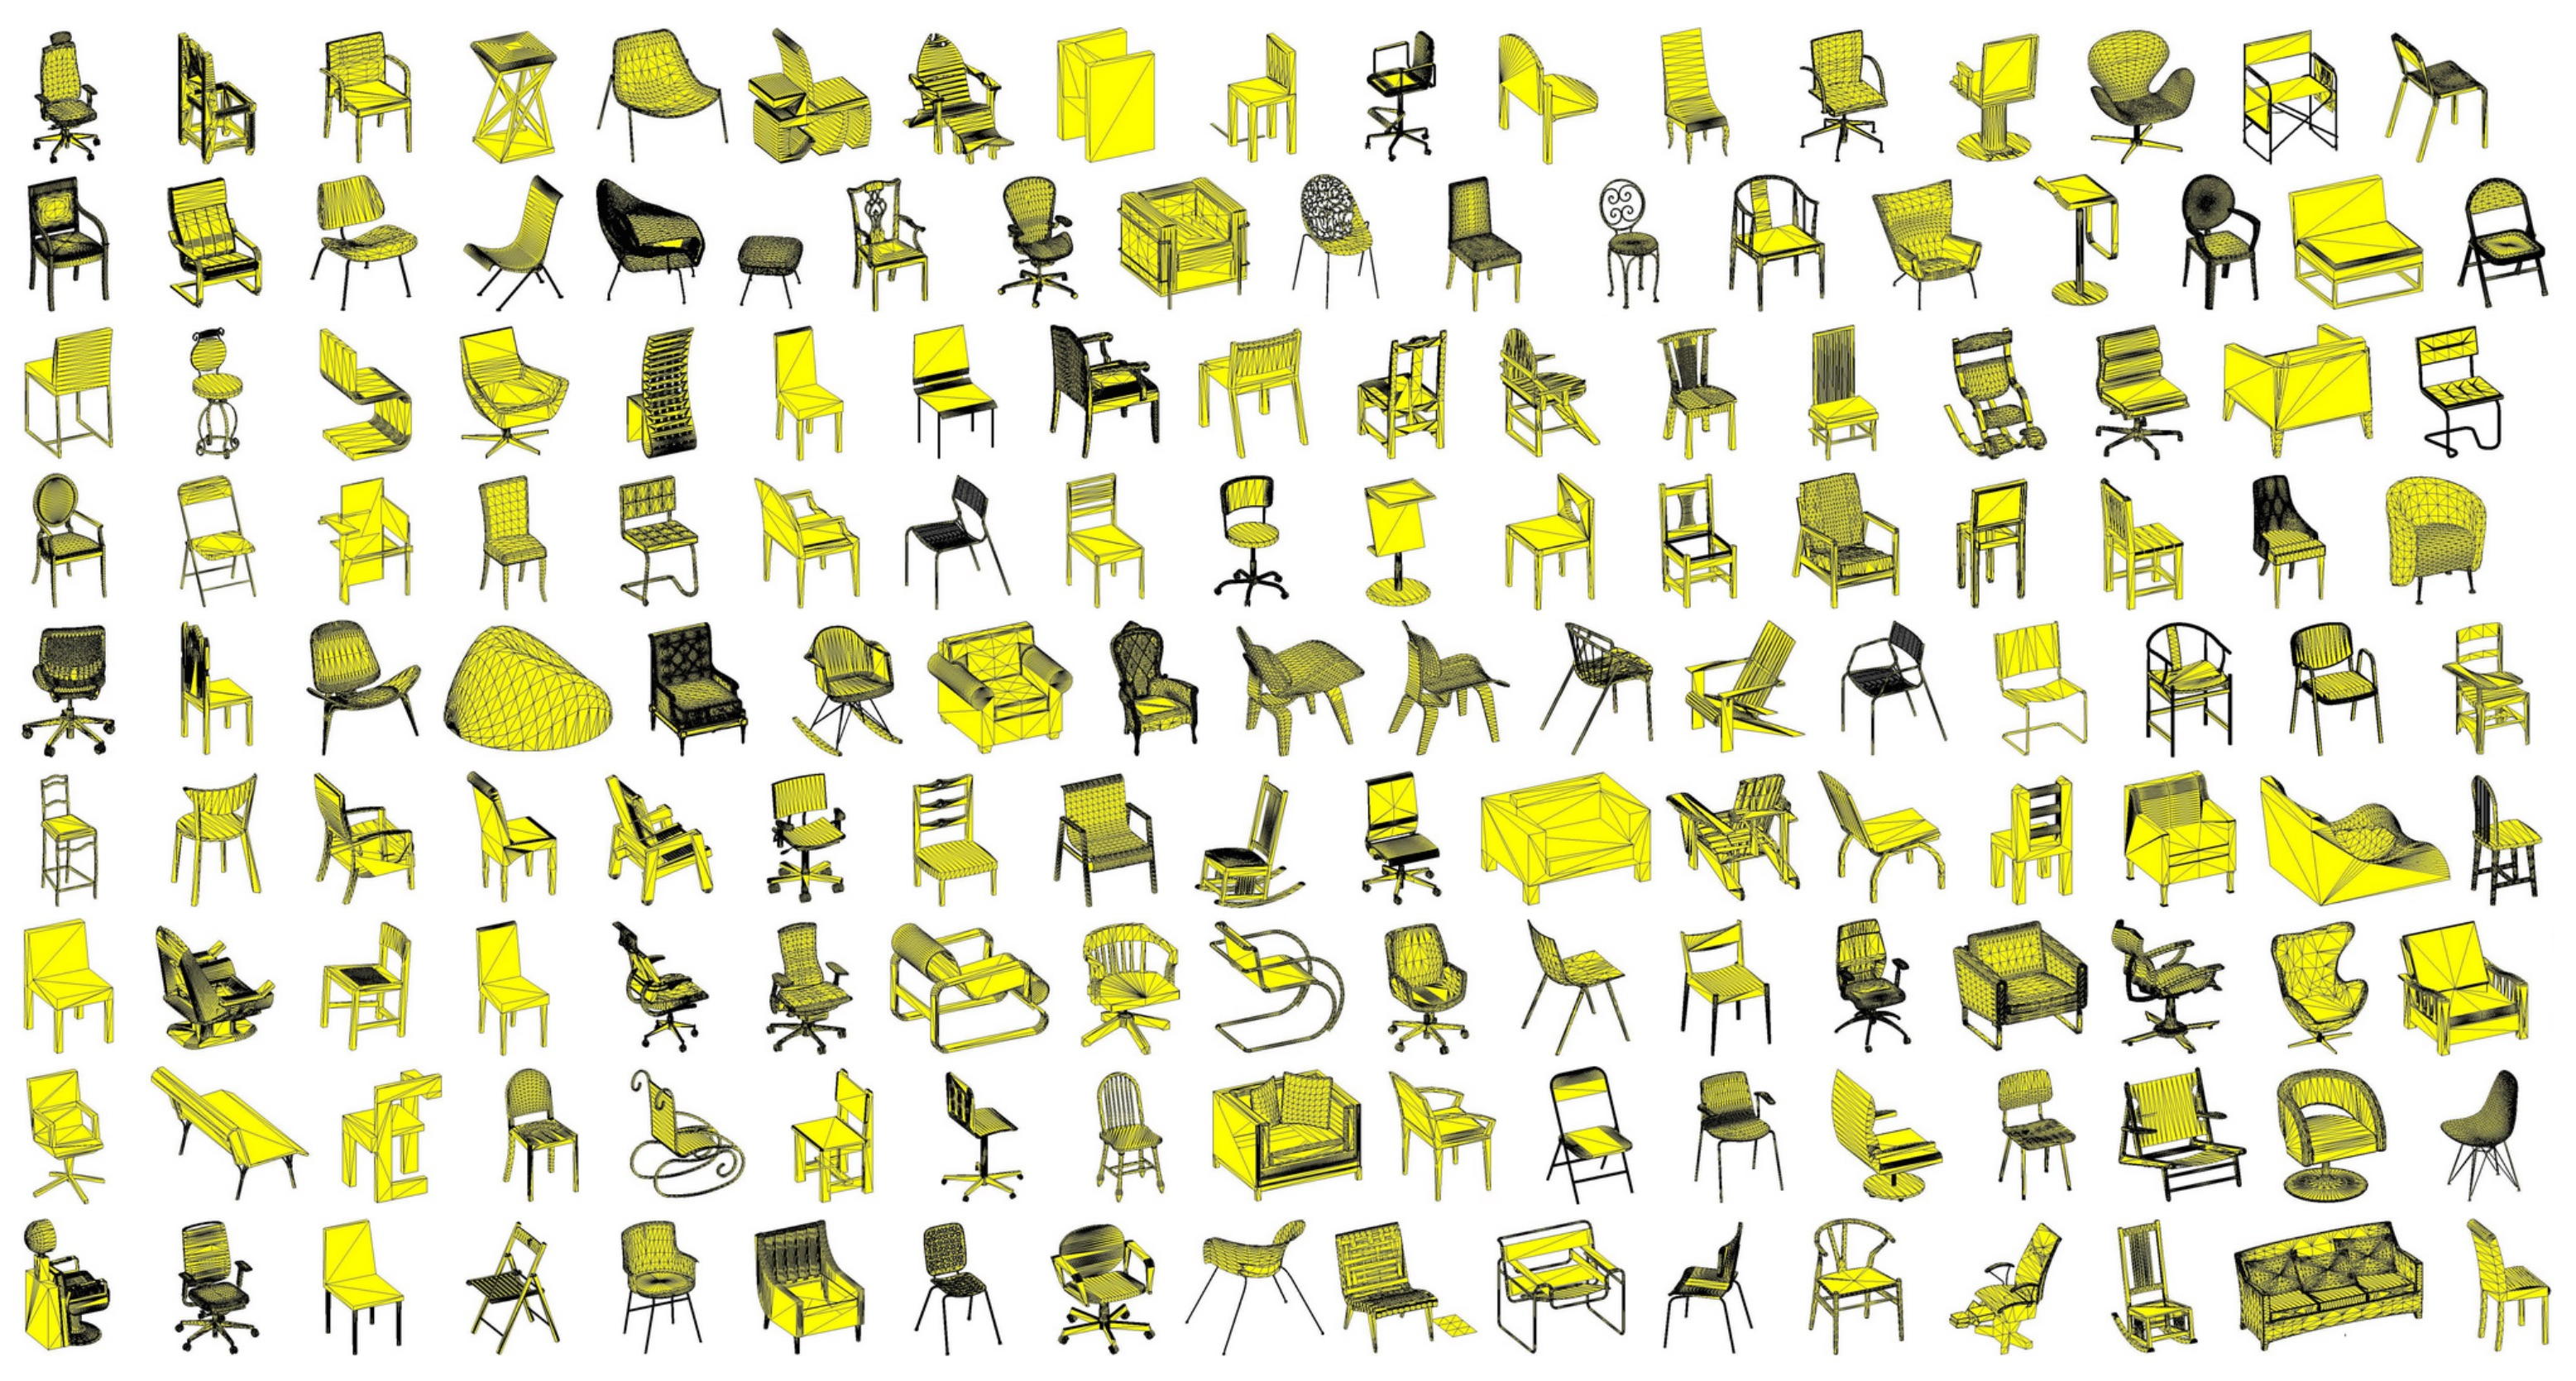
\includegraphics[width=\linewidth]{images/ModelNet.jpg}
\caption{Some of the \emph{chairs} CAD meshed in ModelNet40 \cite{shapenet}.}
\label{fig : modelnet}
\end{figure}
\subsection{Traversability Estimation}
In our Master Thesis work, we trained a convolution neural network to predict the traversability of a ground region for a legged crocodile-like robot called \emph{Krock}. Our approach follows the pipeline proposed by R. Omar Chavez-Garcia et all \cite{omar} where the dataset is entirely generated using synthetic maps in a simulated environment. Figure \ref{fig: hm} shows some of the thirty synthetic heightmaps used in the data generation process. We load those maps into a simulator and spawn the robot on them. Then, we let it walk for a certain amount of time, around $10-20$s, while storing its pose, position and orientation, at a rate of $50hz$. Later, those pieces of information are used to crop around the robot a region of ground, a patch, and compute the advancement for each one of them by projecting the robot pose in the future using a time window, $\Delta t$, of two seconds. Finally, we select a threshold, $tr$, of twenty centimeters to label each patch as \emph{traversable} or \emph{not traversable} if the advancement is major or less respectively. 

The following image shows the patch cropping operation, in each region, we include the robot's footprint and the ground ahead corresponding to the maximum distance it can travel in the selected $\Delta t$.
\begin{figure}[H]
  \centering
      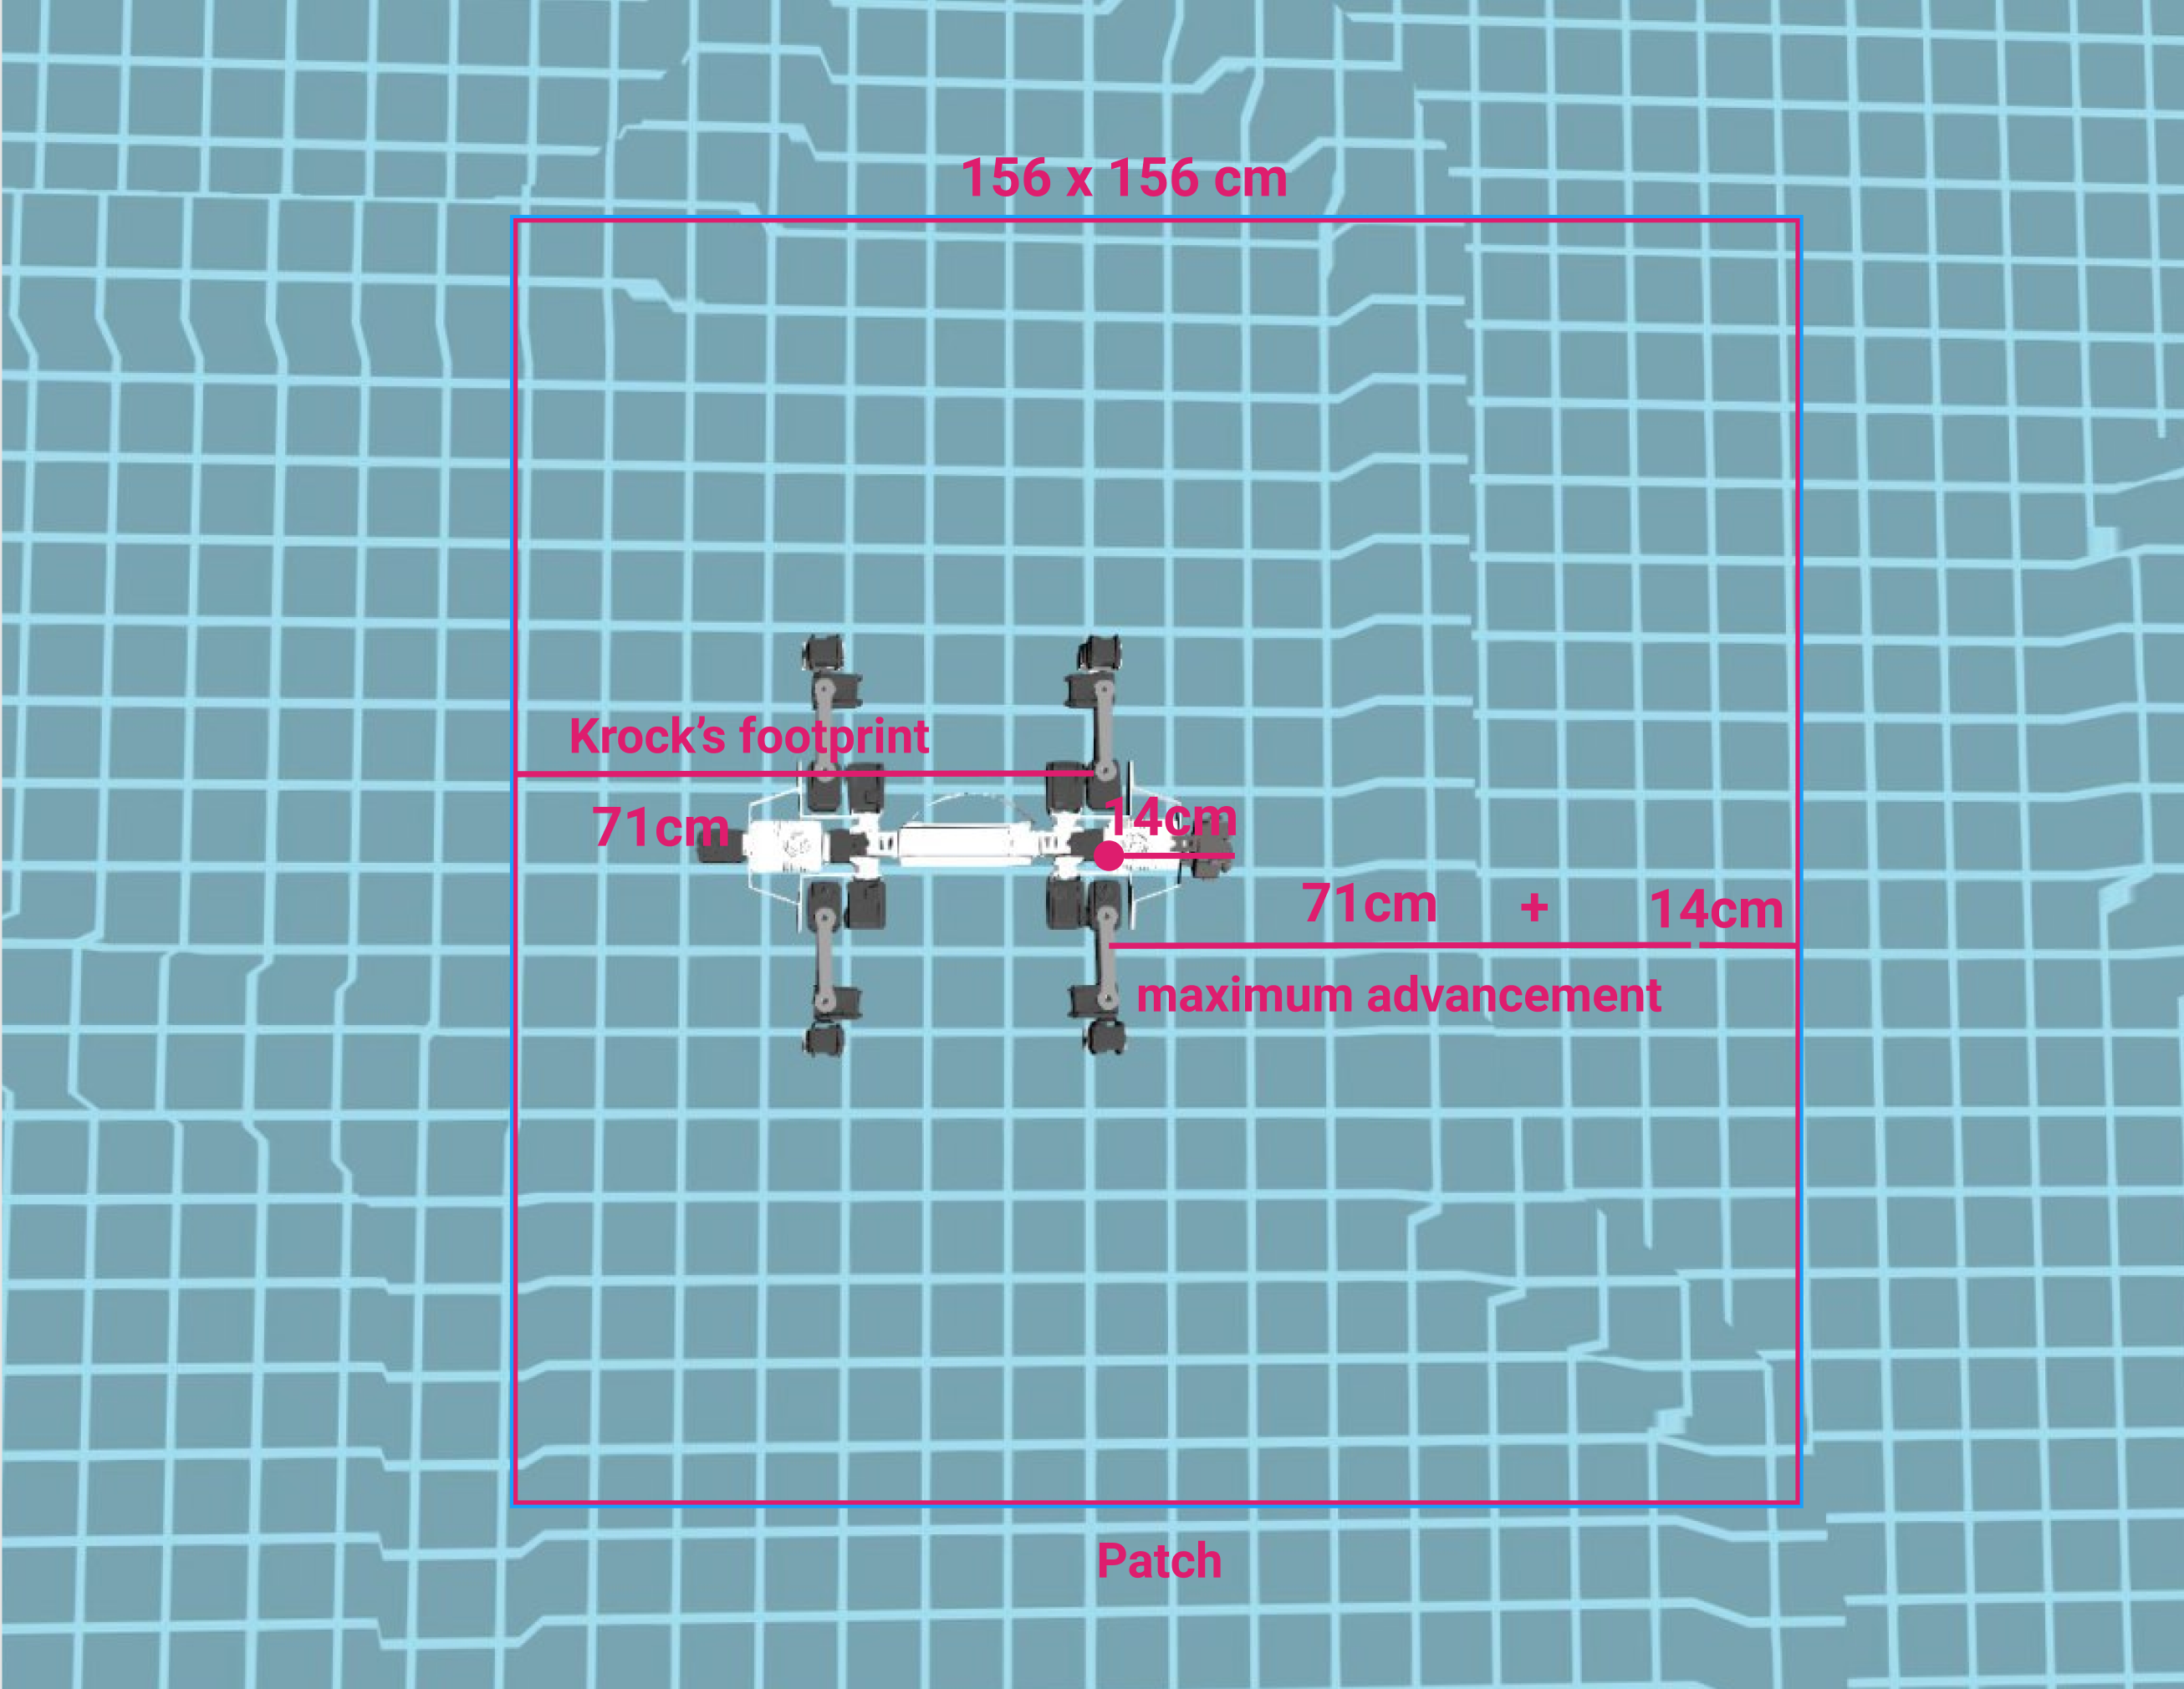
\includegraphics[width=\linewidth]{images/crop/crop.png}
      \subcaption{Robot in the simulator.}
      \begin{minipage}[t]{0.4\linewidth}
      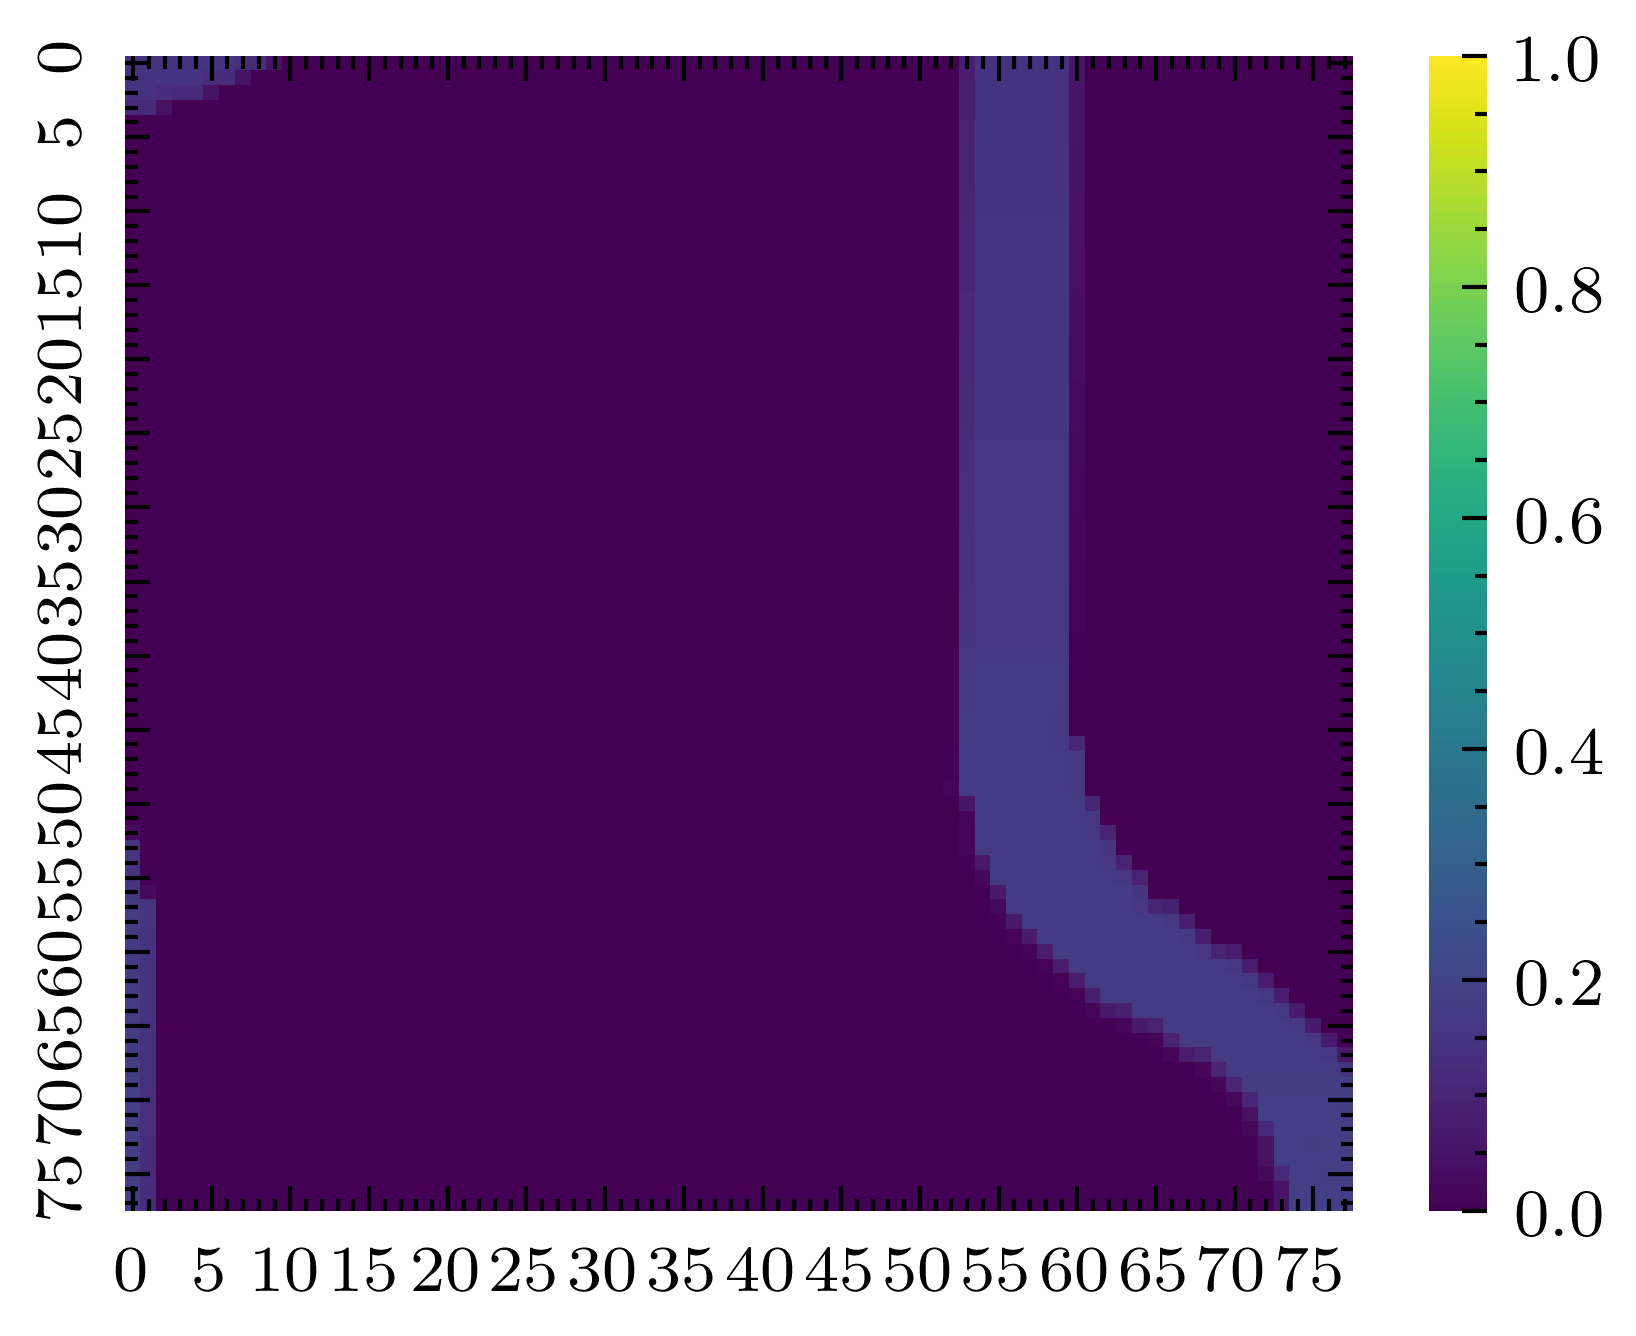
\includegraphics[width=\linewidth]{images/crop/test-1-2d.png}
      \subcaption{Cropped patch in 2d.}
    \end{minipage}
      \begin{minipage}[t]{0.4\linewidth}
      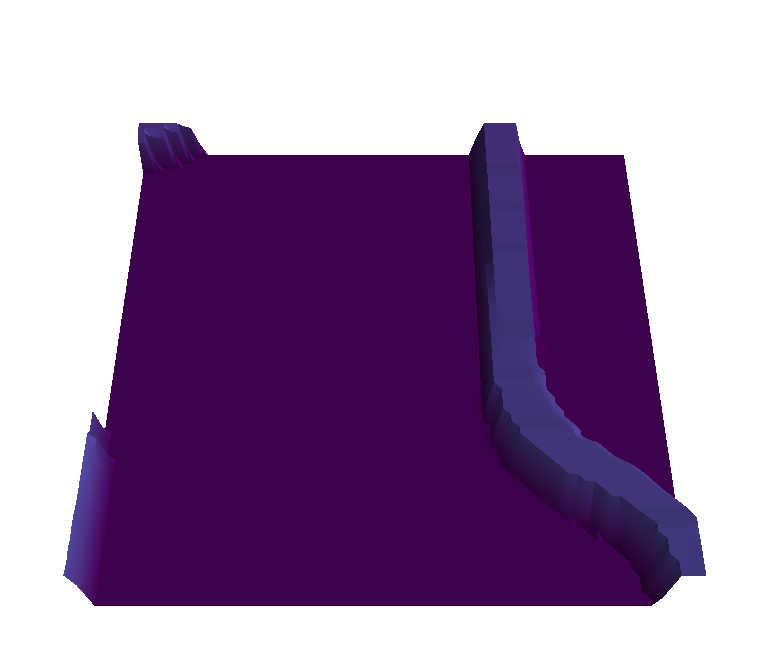
\includegraphics[width=\linewidth]{images/crop/test-1-3d.png}
      \subcaption{Cropped patch in 3d.}
    \end{minipage}
\caption{Patch extract process. Each patch includes the robot's footprint and the maximum ground's region it can traverse in a selected $\Delta t$.}
\end{figure}
\begin{figure*}
  \centering
        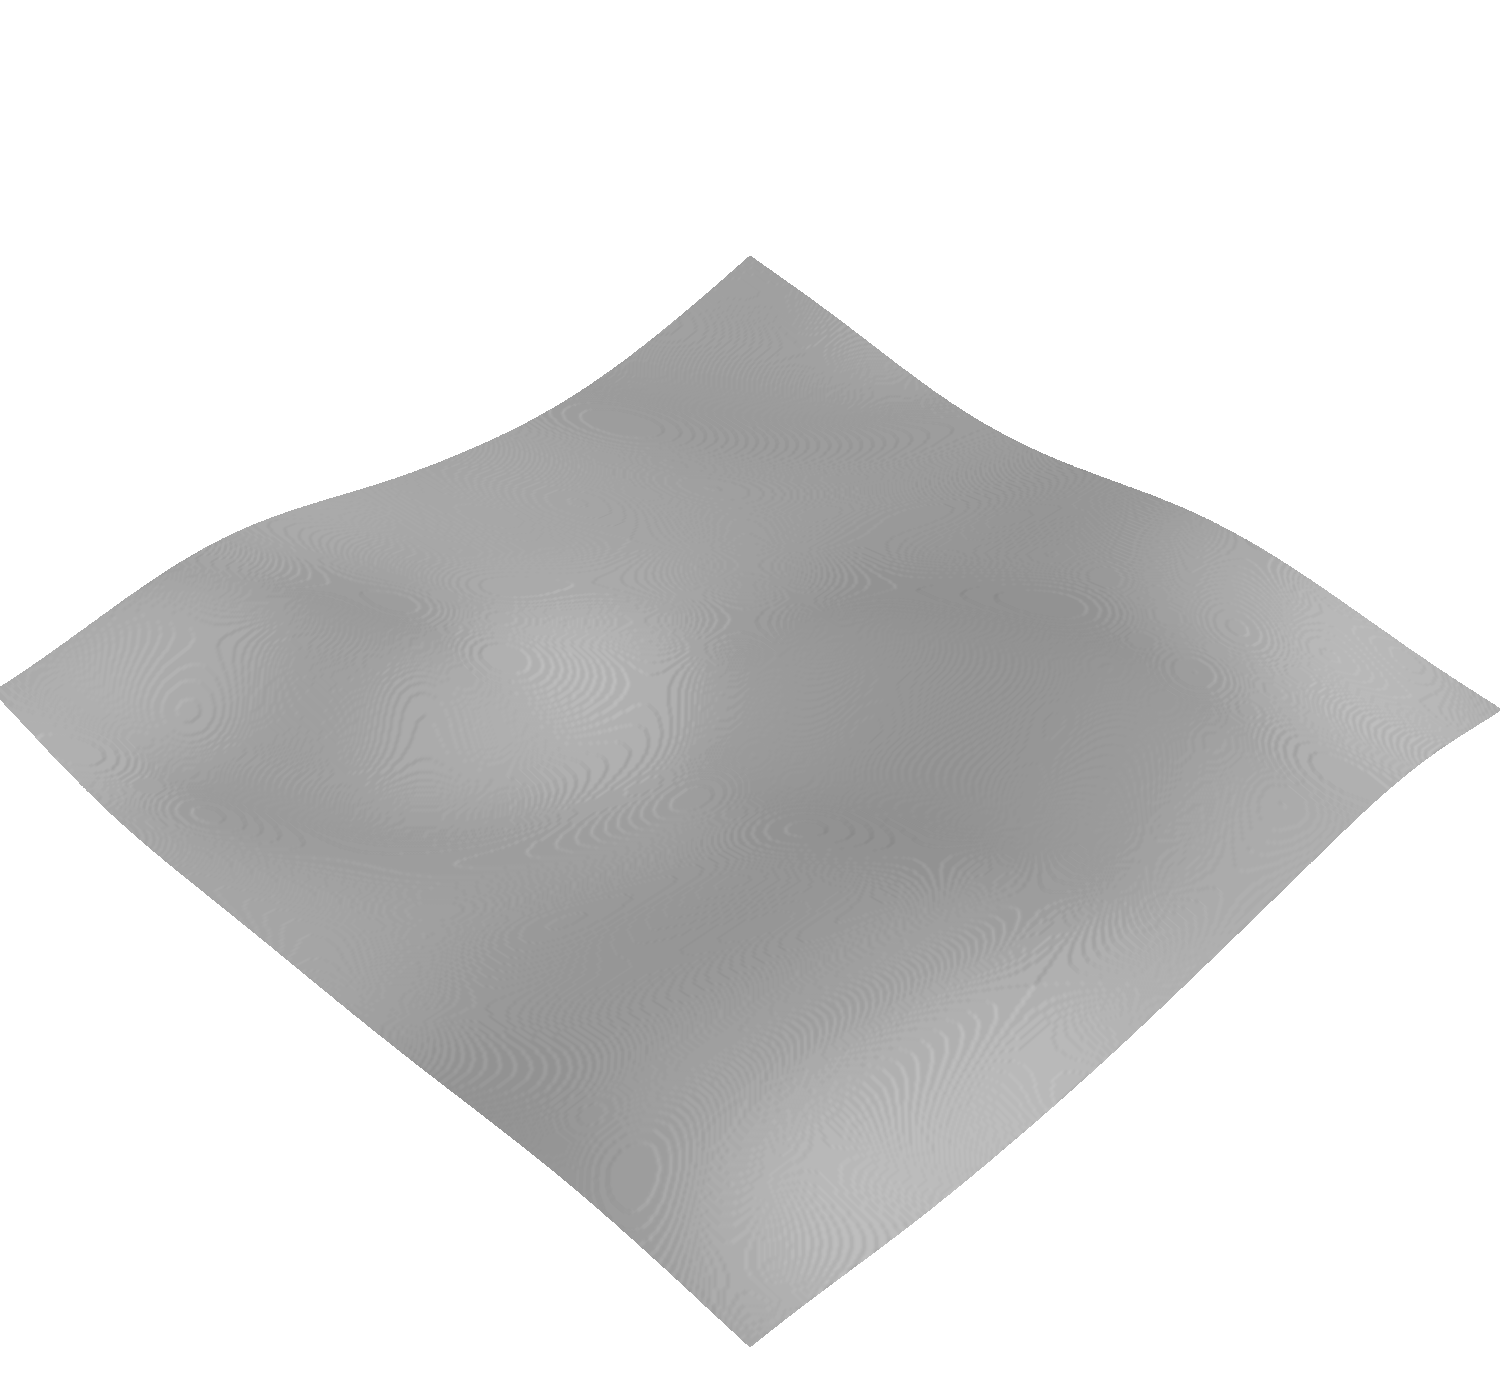
\includegraphics[width=0.22\linewidth]{images/hm3d/bumps0.png}
        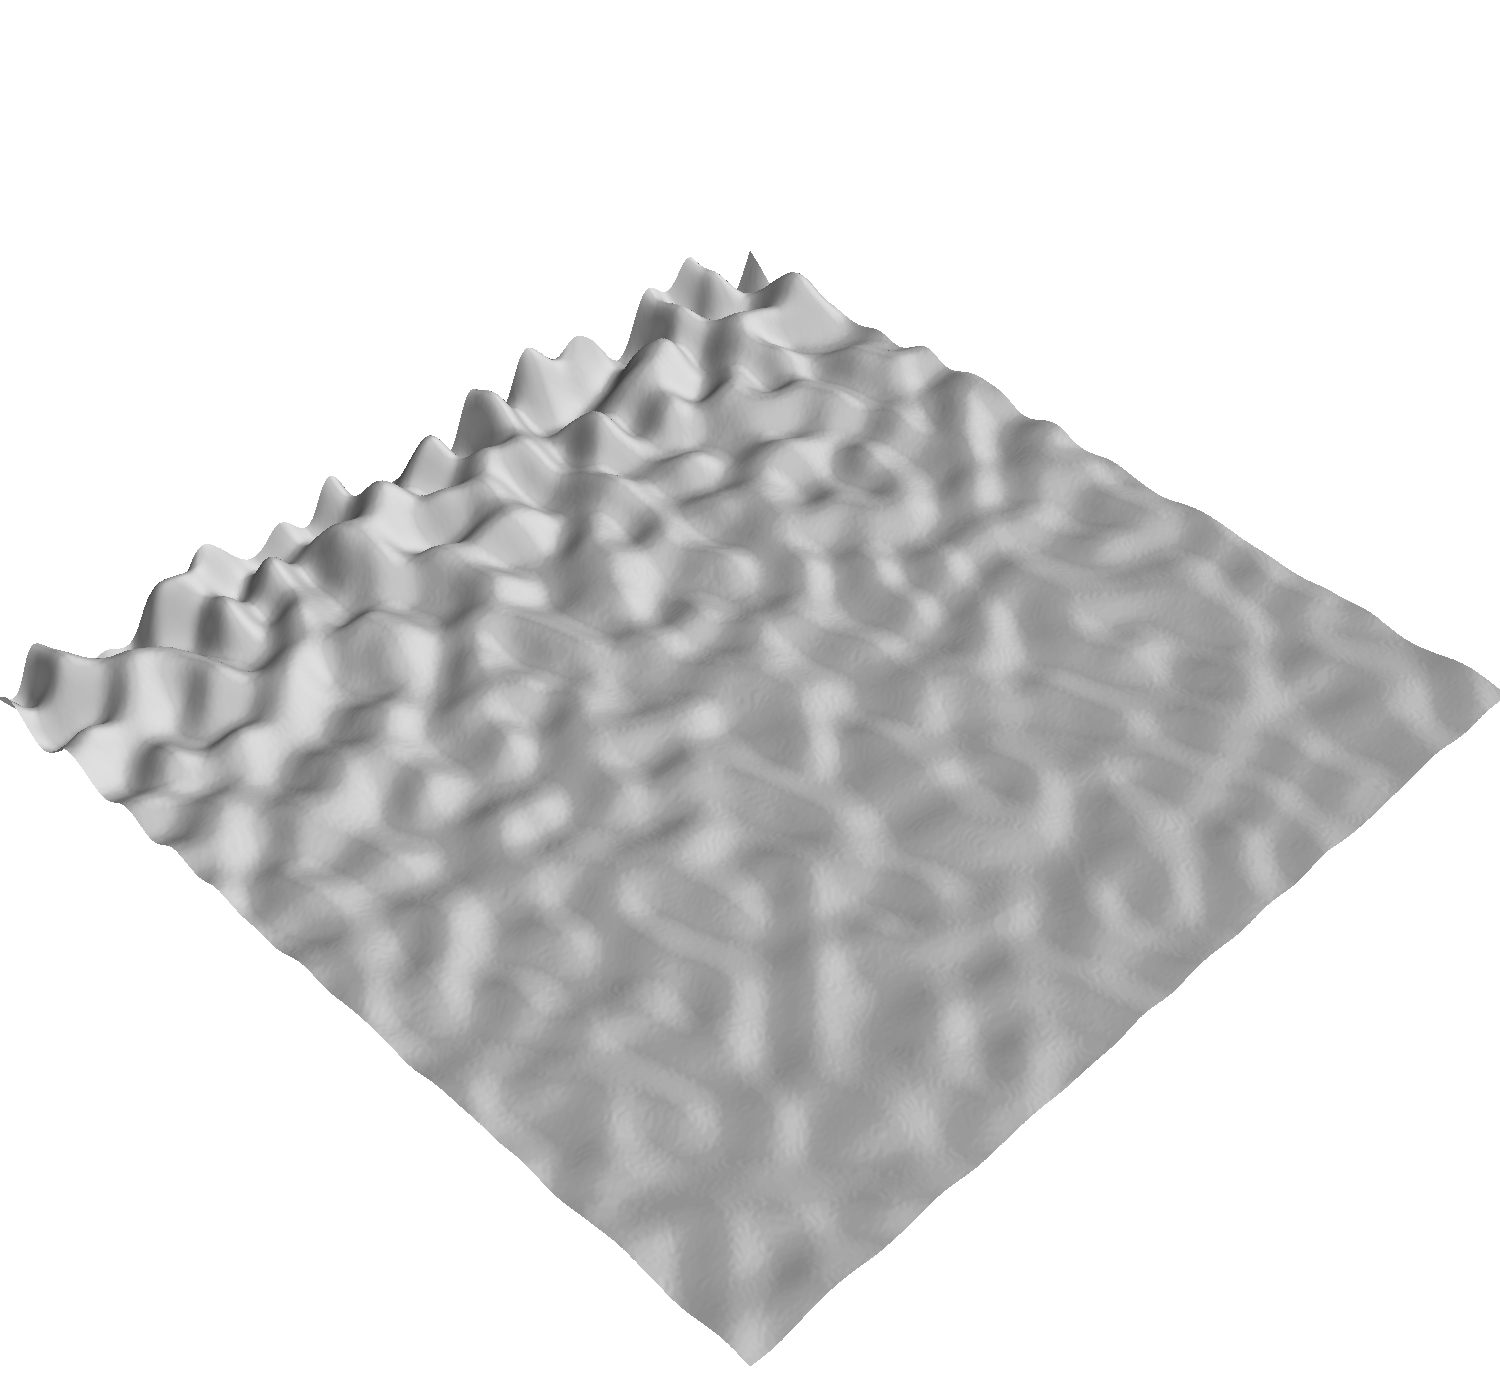
\includegraphics[width=0.22\linewidth]{images/hm3d/bumps3.png}
        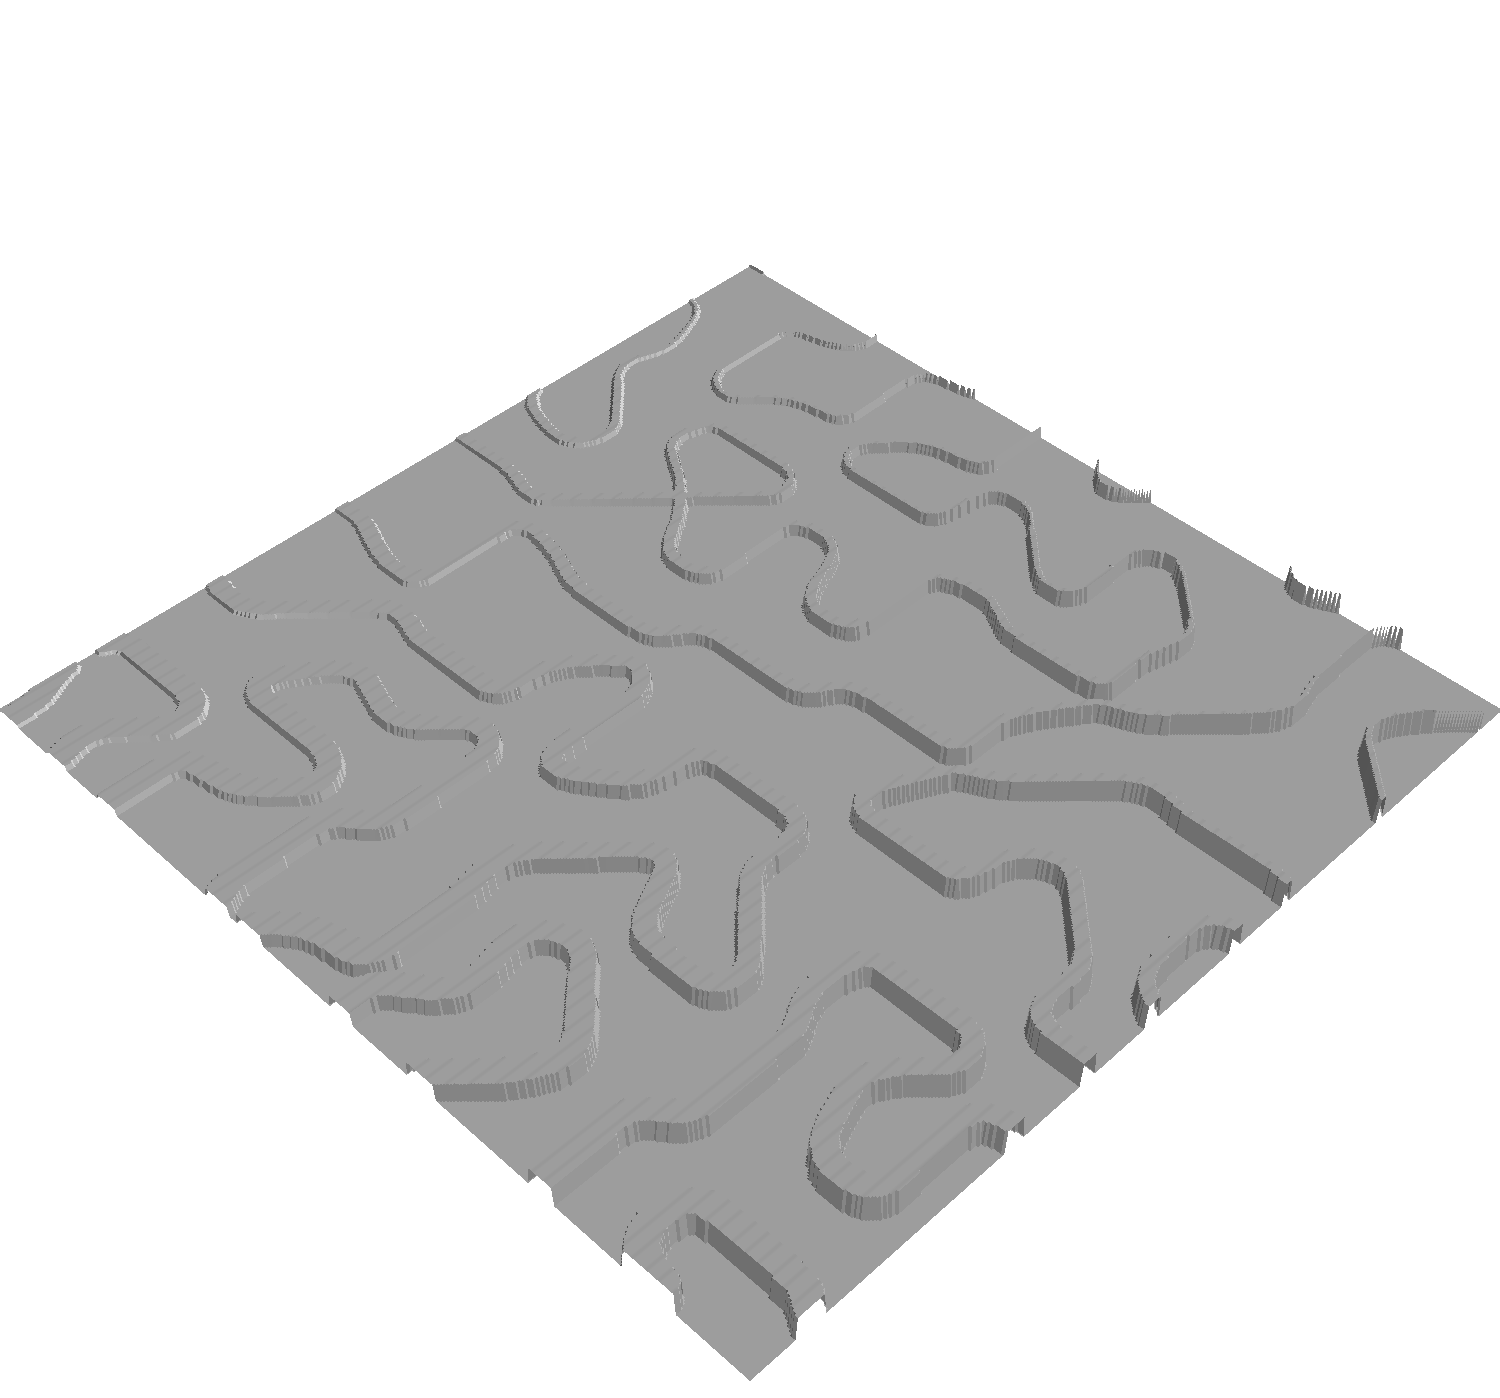
\includegraphics[width=0.22\linewidth]{images/hm3d/bars1.png}
        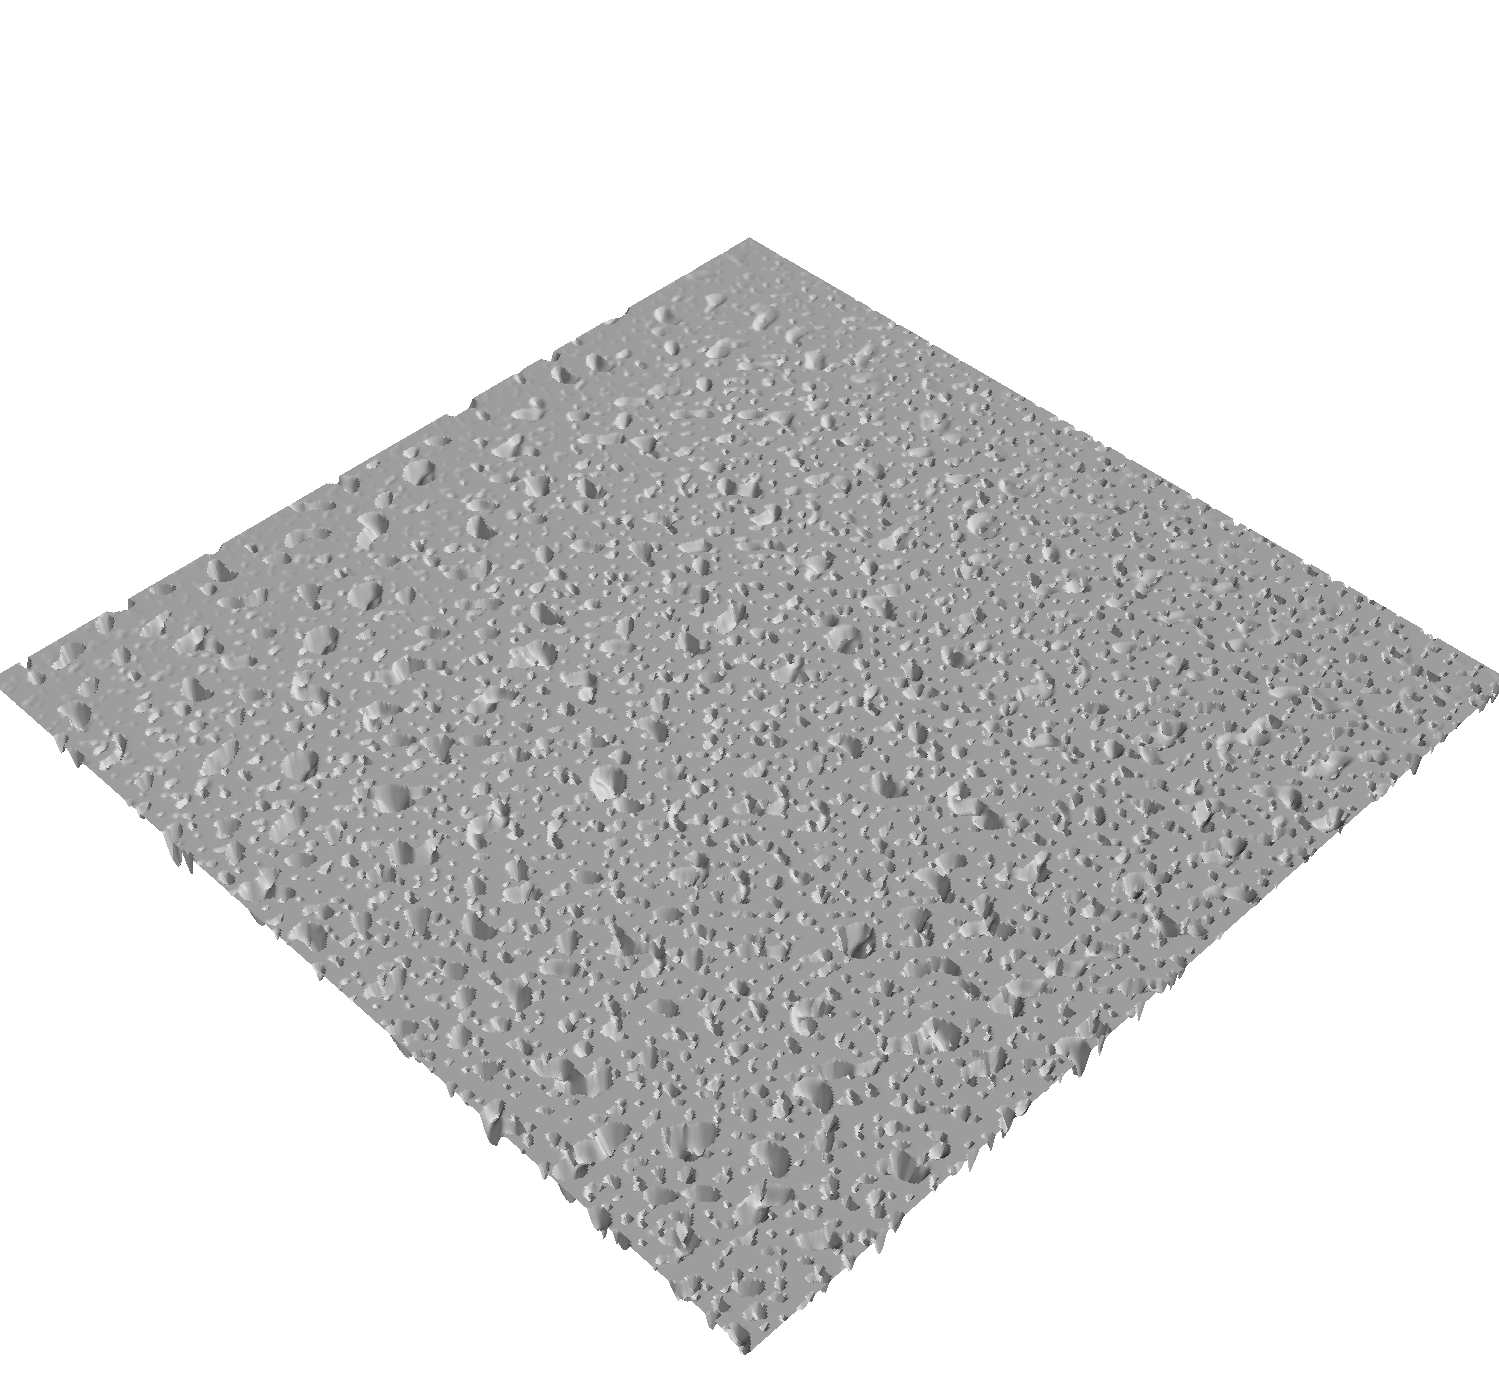
\includegraphics[width=0.22\linewidth]{images/hm3d/holes1.png}
  \caption{Some of the thirty synthetic generated heightmaps, they include bumps, walls and holes. Those maps are loaded into the simulator and we store the robot interactions on them by let it walk forward for a certain amount of time.}
  \label{fig: hm}
  \end{figure*}
\section{Results}
\subsubsection{ModelNet40}
The following table shows the result of the ModelNet40 dataset comparing the original DGCNN and our implementation

\begin{table}[H]
  \centering
  \begin{tabular}{lcc}
    & ACCURACY \\
    \hline
    Original & $92.2$\%  \\
    \textbf{Ours} & $92.0$\%  \\
    \hline
  \end{tabular}
  \caption{Test accuracy score of the original DGCNN and ours implementation on the MonelNet40 dataset.}
\end{table}
Pretrained weights can be downloaded \href{}{here} \todo{todo}
\subsubsection{Traversability Estimation}
We compared the performance of DGCNN against a ResNet \cite{he2015deep} variant on an images dataset for traversability estimation. We kept the same set of hyperparameters used on ModelNet40.
\begin{table}[H]
  \centering
  \begin{tabular}{lcc}
    & ACCURACY \\
    \hline
    MicroResnet & $88.2$\%  \\
    \textbf{DGCNN} & $80.3$\%  \\
    \hline
  \end{tabular}
  \caption{Test accuracy score of a ResNet variant and DGCNN on an images dataset composed of heightmaps for estimate traversability of a legged robot.}
\end{table}
Our CNN has only $314,282$ parameters with a  forward time of $2.41MB$, while DGCNN, in its ideal setup, such has on ModelNet40 dataset, has a forward time of $11MB$ that is comparable with ResNet18. 
\section{Discussion}
Dynamic Graph CNN is a quite elegant architecture to booth classify and segment point cloud. We find it to be very stable during training, similar to CNN . Moreover, it can be easily customizable by changing the size of the EdgeConv and stacking more layers allowing to engineer different models for different tasks.

During our experiments, we also half of the dense layer that maps the features extracted by the two EdgeConv to a bigger space to see how performance will change by bottlenecking the architecture. Surprisingly, the training was very stable and the model's accuracy scored over $90\%$. 

We also train DGCNN on our Master Thesis's dataset composed of images that represent heightmaps. As expected, CNN had a better score and is able to save more memory. However, the DGCNN architecture not parameters hungry and it has a size comparable to a classic ResNet18 used on classic computer vision dataset such as ImageNet \cite{imagenet}. Obviously, it shines on non-euclidean data like point clouds while on images a classic CNN is a better option.

\section{Conclusion}
We successfully reproduced the results of the original on the MonelNet40 reimplemmenting DGCNN entirely in PyTorch. 
\newpage
\bibliography{bib}
\end{document}